%%%%%%%%%%%%%%%%%%%%%%%%%%%%%%%%%%%%%%%%%%%%%%%%%%%%%%%%%%%%%%%%%%%%%%%%%%%%%%%%
% ScaleNav -- ICRA-style manuscript draft
% Compile with ./build.sh
%%%%%%%%%%%%%%%%%%%%%%%%%%%%%%%%%%%%%%%%%%%%%%%%%%%%%%%%%%%%%%%%%%%%%%%%%%%%%%%%

\documentclass[letterpaper,10pt,conference]{ieeeconf}
\IEEEoverridecommandlockouts
\overrideIEEEmargins

\usepackage{amsmath}
\usepackage{amssymb}
\usepackage{booktabs}
\usepackage{graphicx}
\usepackage{xcolor}
\usepackage{placeins}

\newcommand{\vect}[1]{\boldsymbol{#1}}
\newcommand{\mat}[1]{\mathbf{#1}}
\newcommand{\R}{\mathbb{R}}
\newcommand{\blank}{--}

\title{\LARGE \bf
ScaleNav: Semantic Foresight on Persistent Free-Space Graphs\\
for Vision-Based Aerial Navigation
}

\author{First Author$^{1}$ and Second Author$^{2}$%
\thanks{This work was not supported by any organization.}%
\thanks{$^{1}$First Author is with the Affiliation,
        {\tt\small first.author@example.com}}%
\thanks{$^{2}$Second Author is with the Affiliation,
        {\tt\small second.author@example.com}}%
}

\IEEEaftertitletext{%
  \begin{center}
  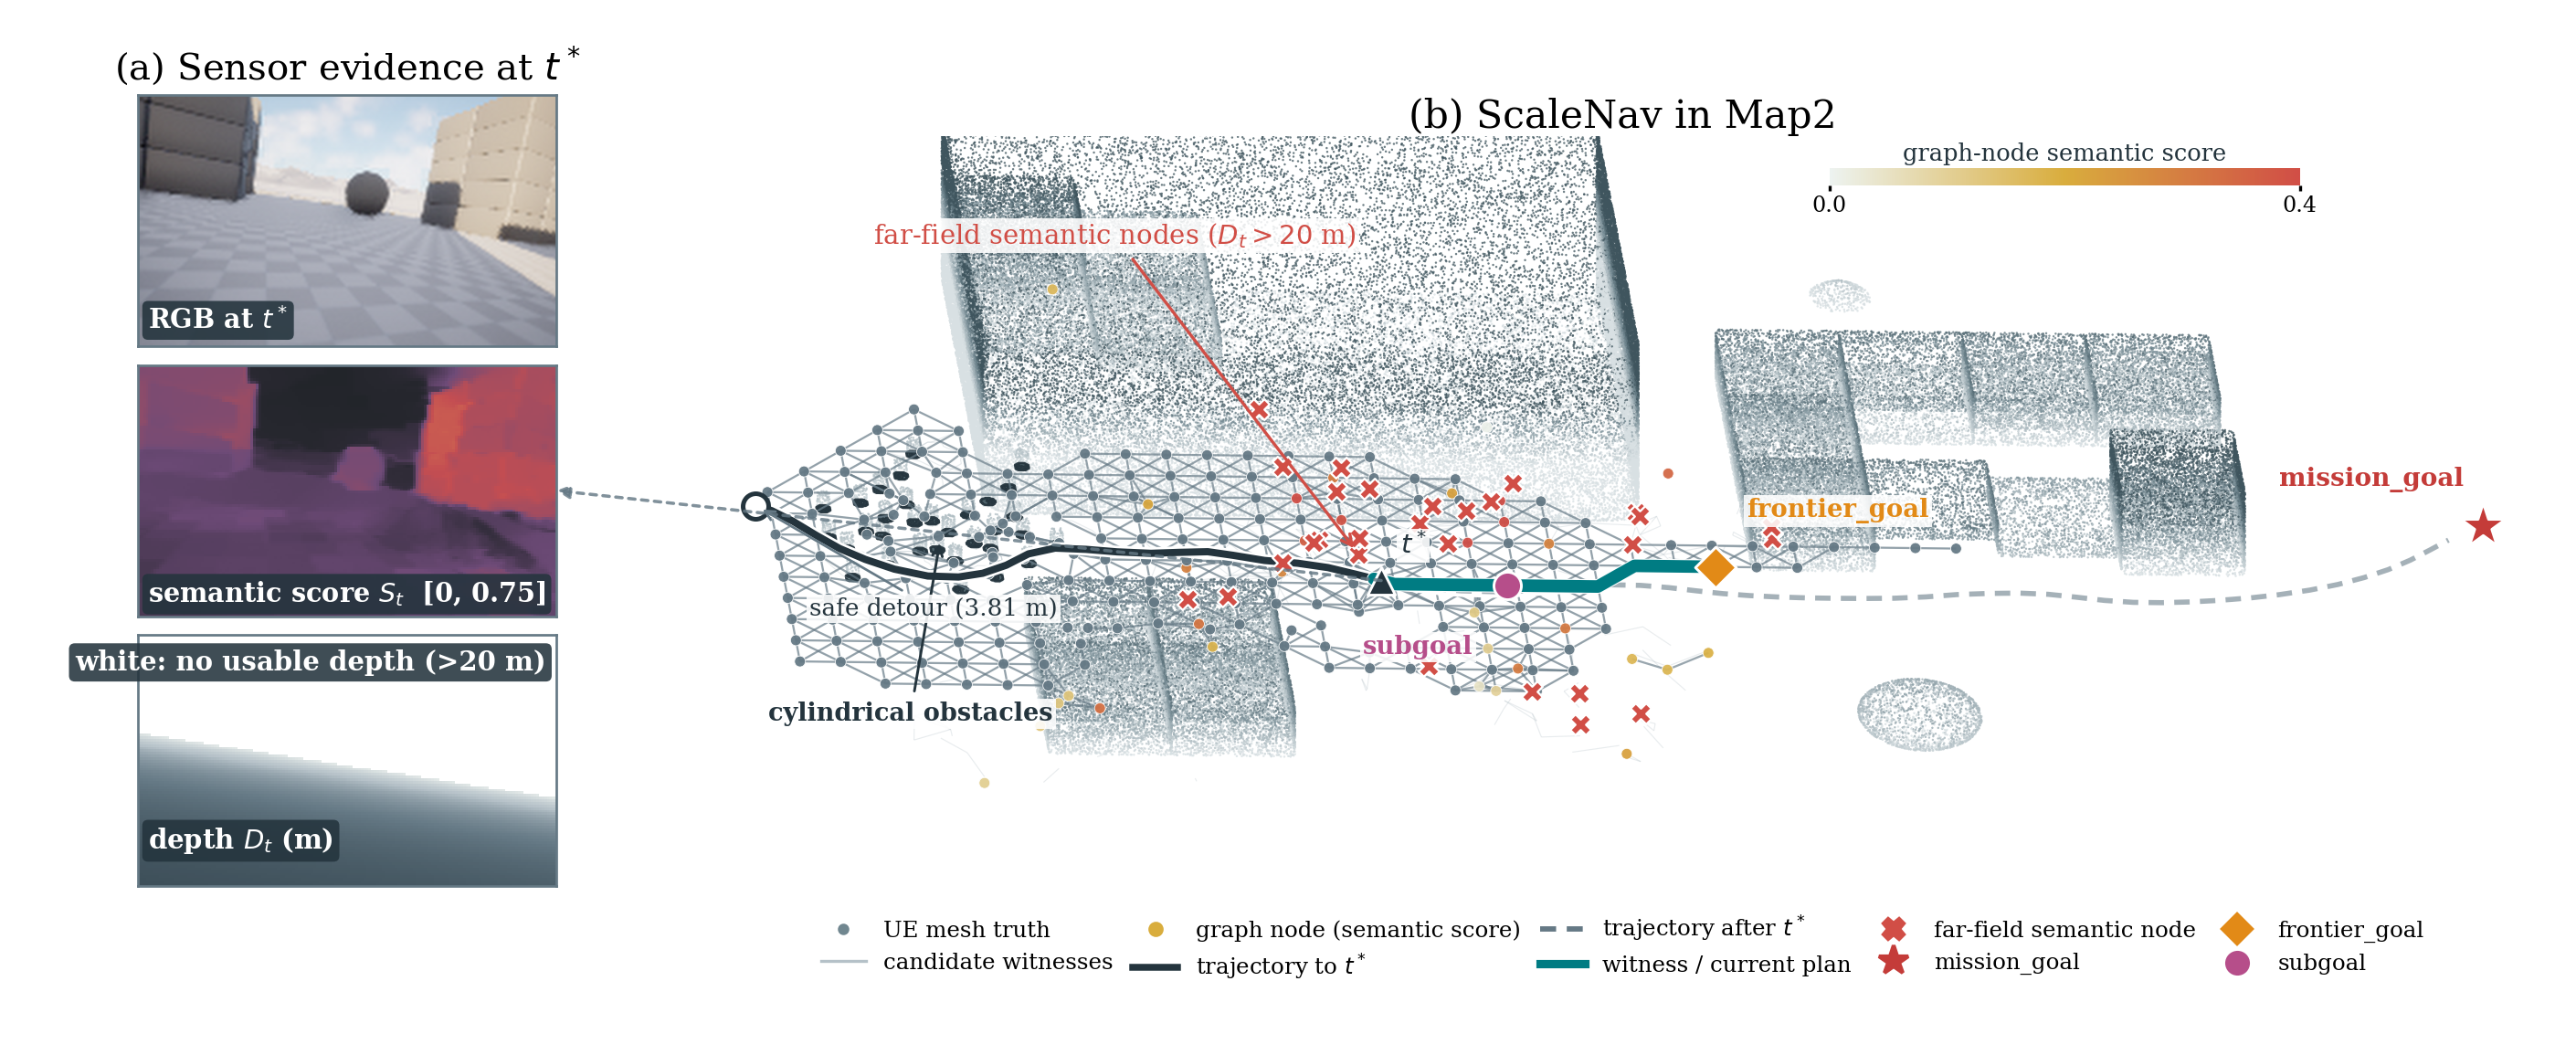
\includegraphics[width=0.98\textwidth]{pics/teaser.pdf}
  \vspace{3pt}
  \parbox{0.98\textwidth}{\footnotesize
  \textbf{Fig. 1.}~ScaleNav in Map2 at synchronized evidence time $t^*$.
  (a)~RGB, semantic score, and depth show semantic response where
  depth is clipped beyond $20$~m. (b)~A shallow aerial view of the mission over
  surface-sampled UE mesh truth. Graph-node fill encodes each node's semantic
  score; crosses mark far-field semantic-node
  positions that lie within the planner's three-dimensional influence radius
  of this graph slice. The persistent graph is shown in a $\pm2$~m
  navigation-height slice. The
  graph/path state is within $90$~ms of $t^*$.
  $mission\_goal$, $frontier\_goal$, and $local\_goal$ denote the task,
  route, and execution layers. Semantics changes route preference but never
  geometric validity.}
  \end{center}%
  \setcounter{figure}{1}%
}

\begin{document}
\maketitle
\thispagestyle{empty}
\pagestyle{empty}

%%%%%%%%%%%%%%%%%%%%%%%%%%%%%%%%%%%%%%%%%%%%%%%%%%%%%%%%%%%%%%%%%%%%%%%%%%%%%%%%
\begin{abstract}
A reactive flight policy can avoid nearby obstacles, but it cannot remember a
detour around a long wall or use semantic evidence beyond valid depth.
ScaleNav adds this missing route-level memory to a neural local planner.  A
bounded graph stores collision-checked free-space bubbles and witness paths.
A frozen open-vocabulary model provides sparse image-space risk observations.
Measured observations update graph nodes, while depth-clipped observations
become persistent far-field hypotheses.  Each hypothesis induces a continuous
risk field on nearby witness paths, allowing an early branch decision without
changing geometric validity.  The selected witness is stored in world
coordinates and remapped after asynchronous graph updates, which preserves
route identity without stale node pointers.

The accepted witness is converted into an ordered local corridor.  A
corridor-conditioned local policy receives this corridor together with depth,
motion, and the frontier goal, then generates a dynamically feasible primitive
inside the committed route.  The topological layer also publishes a 10-m local
goal for execution.  Thus ScaleNav adds long-horizon memory and
language-conditioned route preference without an occupancy grid or ESDF.  On
an independent 1,800-route single-step offline benchmark, corridor conditioning
reduces collision rate from $7.78\%$ to $0.33\%$ and corridor violation from $54.33\%$ to
$8.67\%$, while average progress changes from $6.117$~m to $4.230$~m.
\end{abstract}

%%%%%%%%%%%%%%%%%%%%%%%%%%%%%%%%%%%%%%%%%%%%%%%%%%%%%%%%%%%%%%%%%%%%%%%%%%%%%%%%
\section{INTRODUCTION}
Autonomous flight in an unknown environment requires a quadrotor to solve two
planning problems at once.  It must react to branches and narrow gaps in the
current depth image.  It must also remember which side of a large obstacle
leads toward a distant goal.  The first task calls for a fast local policy;
the second calls for persistent spatial structure.

One-stage neural planners map depth, motion state, and a relative goal to
short, dynamically feasible trajectories \cite{yopo}.  Their planning horizon
is bounded by the current sensing range.  A long wall can therefore force an
early left-or-right
decision whose consequence is invisible in one frame.  Open-vocabulary
perception creates a second mismatch.  An RGB model may recognize a risky
structure beyond valid depth, but a reactive policy has no persistent state in
which to store or use that evidence.

We present ScaleNav, a route-level system that resolves both mismatches.  Depth
builds a persistent graph of free-space bubbles connected by
collision-checked witness paths.  Open-vocabulary image evidence becomes a
continuous risk field on those paths.  A depth-clipped semantic ray creates a
far-field node at a fixed optical depth.  Its distance to each witness changes
route cost before the risk enters the depth range.  The topological planner
then commits an accepted witness and a frontier goal.  The witness is converted
into a fixed number of safe corridor bubbles and passed to a corridor-
conditioned local policy with depth, motion, and the frontier goal.  The topological
planner selects the route; the local policy selects the executable primitive
inside that route.

The separation between semantics and geometry is deliberate.  ScaleNav does
not label an edge safe or unsafe, and it does not feed a semantic heatmap
directly to the policy.  Semantics only ranks collision-valid branches.
Geometric collision checking remains the sole source of validity.  A semantic
error may select a poor route, but it cannot certify an occupied edge as free.

Route persistence is also independent of the current graph representation.
The graph is rebuilt asynchronously as new depth arrives, so node addresses
and local clusters may change while the physical corridor remains valid.
ScaleNav stores the accepted witness in the world frame, remaps a forward
window to the new graph, and applies a soft route prior.  Hysteresis suppresses
unnecessary branch changes, while a risk-triggered release preserves the
ability to replan when new evidence changes the route preference.

The main contributions are:
\begin{itemize}
  \item \textbf{Semantic foresight on free-space topology.}
  Open-vocabulary evidence is represented as a continuous risk field over
  collision-checked witness paths, enabling early branch selection without
  changing geometric validity.
  \item \textbf{Persistent far-field semantic nodes.}
  Depth-clipped observations become bounded, graph-connected hypotheses at a
  fixed optical depth and are promoted when measured bubbles reach them.
  \item \textbf{Route identity across graph replacement.}
  A world-frame witness and hysteretic route gate preserve the incumbent route
  across asynchronous topology updates without stale node pointers.
  \item \textbf{Corridor-conditioned local execution.}
  An accepted witness becomes an ordered corridor for a corridor-conditioned
  local policy, which generates dynamics-aware primitives without an occupancy
  grid or ESDF.
\end{itemize}

We evaluate the complete route contract in paired simulation experiments and
report the current offline corridor-conditioned benchmark.  The experiments
separate
topology, semantic foresight, route stability, local route adherence, and
system cost.  The model-independent semantic contract also permits a larger
VLM, such as Qwen3-VL, to replace PEARL without changing graph search.

\begin{figure*}[t]
\centering
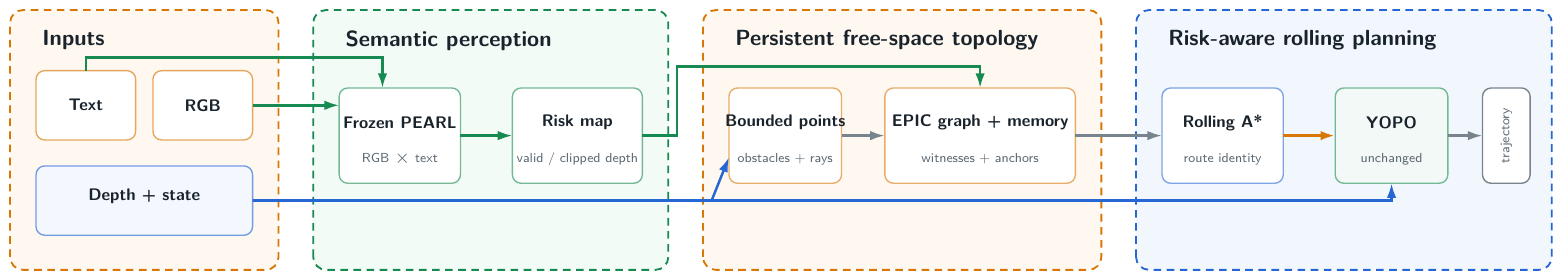
\includegraphics[width=0.98\textwidth]{pics/system_architecture_paper.pdf}
\caption{ScaleNav system architecture. Depth builds Bubble topology and
collision-checked edge witnesses. RGB and the text query produce patch scores
that are projected at fixed optical depth into persistent graph-node semantic
state; later Bubble overlap promotes an \texttt{Unknown} semantic node to
\texttt{Verified}. Continuous witness risk enters rolling A* and the route
gate, which maintain \texttt{frontier\_goal} and the accepted witness. A
10-m lookahead on that witness produces \texttt{local\_goal}, while ordered
witness corridor bubbles are extracted from the accepted witness and passed to
a corridor-conditioned local policy. Semantics changes route cost but cannot create or
validate an edge.}
\label{fig:architecture}
\end{figure*}

%%%%%%%%%%%%%%%%%%%%%%%%%%%%%%%%%%%%%%%%%%%%%%%%%%%%%%%%%%%%%%%%%%%%%%%%%%%%%%%%
\section{RELATED WORK}
\subsection{Local Reactive Flight}
Depth-based reactive planners trade global consistency for low latency.
RAPPIDS partitions a single depth image into rectangular pyramids and tests
candidate trajectories against them \cite{rappids}.
NanoMap keeps a short history of raw range measurements and answers
uncertainty-aware proximity queries without fusing a global map
\cite{nanomap}.
EGO-Planner removes the ESDF from the local optimization loop
\cite{egoplanner}, and learned policies collapse sensing, search, and
optimization into a single network pass \cite{yopo,loquercio}.
Classical quadrotor systems combine kinodynamic search with online collision
checking; Fast-Planner emphasizes efficient polynomial replanning in unknown
3-D space \cite{fastplanner}, while FASTER separates a safe graph search from
trajectory optimization under limited sensing \cite{faster}.  SUPER pushes this
line further with dual trajectories over point-cloud corridors, demonstrating
safety-assured flight above $20$~m/s in cluttered scenes \cite{super}.
These designs motivate our separation between a route-level witness and the
local primitive.
These methods optimize motion from the current observation or a short local
history.  They do not expose a persistent route state that can remember which
side of a distant wall was selected.  ScaleNav retains their fast reactive role
and adds route memory and semantic preference at a separate layer.

\subsection{Persistent Free-Space Structure}
A second line of work builds structure that outlives one sensor frame.
The frontier formulation of Yamauchi \cite{yamauchi}, the incremental
frontier structure in FUEL \cite{fuel}, and the hierarchical exploration
roadmap of TARE \cite{tare} establish the route-level exploration
view.  OctoMap stores probabilistic occupancy in an octree \cite{octomap},
whereas Voxblox maintains distance-field representations for planning
\cite{voxblox}.
Bubble Planner extends receding safe corridors for
high-speed flight \cite{bubble}.
Prior bubble-graph methods cluster free-space spheres from point clouds into
lightweight topologies for large-scale exploration \cite{epic}.
These structures are geometric: their costs encode distance or information
gain, so a text query such as ``avoid the crowd'' has no representation.
ScaleNav uses the same lightweight free-space abstraction but solves a
different problem.
It performs goal-directed rolling search, preserves a selected witness
route across asynchronous graph replacement, and lets edges carry
open-vocabulary risk while geometric validity remains unchanged.

\subsection{Open-Vocabulary Perception and Semantic Navigation}
Open-vocabulary models supply image evidence beyond a fixed label set.
CLIP aligns image and text embeddings \cite{clip}, and PEARL produces
training-free open-vocabulary segmentation aligned with image geometry
\cite{pearl}.
Language-driven segmentation provides dense text-conditioned masks
\cite{lseg}, while Segment Anything supplies class-agnostic masks that can be
associated with a query by a separate embedding model \cite{sam}.  Recent
open-set 3-D systems such as ConceptFusion and OpenScene lift these signals
into mapped scene representations \cite{conceptfusion,openscene}.
On the planning side, VLFM builds vision-language value maps to select
frontiers for object navigation \cite{vlfm}, RayFronts encodes open-set
semantics on both mapped voxels and beyond-range rays for online
exploration \cite{rayfronts}, and WildOS scores the frontier nodes of a
sparse navigation graph with a vision-language module to search for
open-vocabulary objects beyond the depth horizon \cite{wildos}.
These systems bring semantics into the map or the frontier score, but the
map itself is the product; how a route should bend around a risky region
before the sensor reaches it is left to a separate decision layer.  WildOS
attracts a robot toward a queried object; avoidance instead requires risk to
repel a route, continuously along its length rather than only at its
terminal.  ScaleNav targets exactly this interface: sparse image-space
observations become persistent costs on free-space edges, including evidence
whose depth is clipped, while collision validity remains purely geometric.

%%%%%%%%%%%%%%%%%%%%%%%%%%%%%%%%%%%%%%%%%%%%%%%%%%%%%%%%%%%%%%%%%%%%%%%%%%%%%%%%
\section{PROBLEM FORMULATION}
Let the vehicle state at time $t$ be
$\vect{x}_t=(\vect{p}_t,\vect{v}_t,\vect{a}_t,\vect{R}_t)$.
The sensors provide an RGB image $I_t$, a depth image $D_t$, and
odometry.
The mission gives a world-frame goal $\vect{g}$ and a text query $q$ that
describes regions to avoid.
No prior geometric map is available.

The planner must output a dynamically feasible local trajectory $\tau_t$.
We separate this problem into a slow route decision and a fast motion
decision:
\begin{align}
  (\mathcal{W}_t,\vect{g}^{\mathrm{front}}_t,
   \vect{g}^{\mathrm{loc}}_t)
    &= \Pi_{\mathrm{topo}}(\mathcal{G}_t,I_{0:t},D_{0:t},q,\vect{g}), \\
  \tau_t
    &= \Pi_{\mathrm{local}}(D_t,\vect{v}_t,\vect{a}_t,
       \vect{R}_t^\top(\vect{g}^{\mathrm{front}}_t-\vect{p}_t),
       \mathcal{B}_t).
\end{align}
Here $\mathcal{W}_t$ is the accepted world-frame witness and
$\mathcal{B}_t$ is its fixed-size corridor representation.  The local policy
is a corridor-conditioned local policy.  It receives one $160\times96$ depth channel,
body-frame motion, the frontier goal, and the ordered corridor:
\begin{equation}
 \vect{o}_t = [\vect{v}^{B}_t,\vect{a}^{B}_t,
                (\vect{g}^{\mathrm{front}}_t-\vect{p}_t)^{B}] \in \R^9,
 \qquad
 \mathcal{B}_t\in\R^{12\times4}.
\end{equation}
The $12$ rows contain bubble center and safe radius; a binary route mask marks
valid rows.  The local policy does not create a new frontier or change the global
homotopy.  It chooses a dynamically feasible primitive inside the accepted
route.

The primitive lattice follows the released YOPO parameterization.  The
$160\times96$ depth feature map is decoded on a $3\times5$ grid, giving
$N_{\mathrm{prim}}=15$ candidate directions.  Each candidate predicts a
nine-dimensional terminal state $[\vect{p}_1,\vect{v}_1,\vect{a}_1]\in\R^9$
and one scalar score.  The terminal state is converted to a smooth
polynomial primitive using the fixed-duration boundary-value solver: the
current position, velocity, and acceleration are fixed at the start, while
the predicted terminal derivatives are free.  Candidate selection is thus a
discrete choice over dynamically parameterized primitives, rather than direct
regression of a timed expert path.

For the route-aware variant, each corridor row contributes the body-frame
center, its safe radius, and a validity bit.  The network concatenates the
validity bit with the four geometric values, so the learned route feature has
$12\times5$ scalars even though the geometric corridor itself is
$12\times4$.  Rows beyond the available witness are zero-padded and masked.
When the route contract is invalid or stale, all rows are masked and the
frontier-only YOPO input is recovered.  This explicit zero-input behavior
keeps route conditioning from becoming a hidden safety dependency.

We use a fixed-height planning layer in the current experiments to isolate the
horizontal branch-selection problem.
The depth sensing, point memory, and local trajectory execution remain 3-D.
The proposed semantic cost is defined on 3-D witness polylines and does not
require the fixed-height assumption.

%%%%%%%%%%%%%%%%%%%%%%%%%%%%%%%%%%%%%%%%%%%%%%%%%%%%%%%%%%%%%%%%%%%%%%%%%%%%%%%%
\section{PERSISTENT FREE-SPACE TOPOLOGY}
\label{sec:topology}
\subsection{Bounded Geometric Memory}
Depth is back-projected into obstacle points and free-ray evidence.
The implementation voxel-filters the current frame and retains at most
$N_{\max}$ points; no points from earlier frames are kept in this buffer.
It does not construct occupancy voxels or an ESDF.

Following prior bubble-graph construction \cite{epic}, collision-free bubbles
are clustered into graph vertices.
A vertex is
\begin{equation}
 v_i=(\vect{c}_i,\rho_i,z_i,h_i),
\end{equation}
where $\vect{c}_i$ is its center, $\rho_i$ is free-space clearance, $z_i$ is
semantic state, and $h_i$ is a persistent identity record.
An edge stores a collision-checked witness polyline
\begin{equation}
 \pi_{ij}=\{\vect{w}^{ij}_0,\ldots,\vect{w}^{ij}_{M_{ij}}\},
 \quad
 L_{ij}=\sum_{m=1}^{M_{ij}}
 \|\vect{w}^{ij}_m-\vect{w}^{ij}_{m-1}\|_2.
\end{equation}
The witness is important twice.
It is the executable geometric connection, and it is the support on which
semantic distance is measured.
The chord $\vect{c}_j-\vect{c}_i$ is insufficient because a valid witness may
bend around an obstacle.

Geometry is updated in a background graph.
After local bubble generation, region clustering, and graph connection, an
atomic swap exposes the new graph to planning.
The point budget and spatial radius bound memory.
Transiently missing bubbles receive a short grace period before deletion.

\subsection{Clearance-Aware Edge Cost}
Let $\rho_{ij}=\min(\rho_i,\rho_j)$ and let $\rho^\star$ be the target
clearance.
The implemented soft clearance term is
\begin{equation}
 C_{\mathrm{clr}}(e_{ij})=
 \lambda_{\mathrm{clr}}L_{ij}
 \left[
 \max\left(0,\frac{\rho^\star-\rho_{ij}}{\rho^\star}\right)
 \right]^2.
\label{eq:clearance}
\end{equation}
It prefers open routes but does not declare a narrow valid edge invalid.
Geometric feasibility remains determined by the bubble graph and its witness
checks.

\begin{figure}[t]
\centering
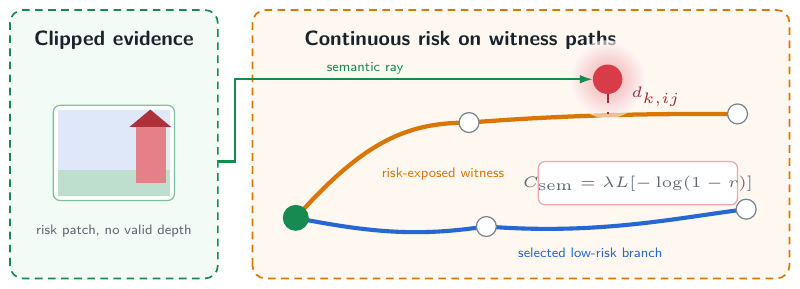
\includegraphics[width=\columnwidth]{pics/semantic_risk_field_paper.pdf}
\caption{Real logged ScaleNav decision in Map2.  The left panel is the logged
RGB frame with the deployed PEARL heatmap and $5\times3$ pooling grid; red
rings identify high responses whose synchronized depth has no return.  The
right panel is the first graph update after this evidence changes the route,
with the logged persistent graph, far-field nodes, witness exposure, and
selected witness.  The panels are synchronized by the recorded evidence and
graph timestamps.  Semantics ranks collision-valid branches and never changes
geometric validity.}
\label{fig:risk_field}
\end{figure}

%%%%%%%%%%%%%%%%%%%%%%%%%%%%%%%%%%%%%%%%%%%%%%%%%%%%%%%%%%%%%%%%%%%%%%%%%%%%%%%%
\section{SEMANTIC FORESIGHT}
\label{sec:semantics}
\subsection{Semantic Observation Model}
The frozen PEARL model maps $(I_t,q)$ to a patch heatmap.
The heatmap is max-pooled on a $5\times3$ grid, and a low-quantile
background baseline is subtracted so that weak whole-image responses do not
become risk.
Every retained patch is projected by the calibrated pinhole model at a fixed
optical-axis depth $\ell_s$, independent of the measured depth:
\begin{equation}
 \vect{y}_{u,t}=\vect{p}_t+\mat{R}_t
 \left(\vect{t}_{\mathrm{cam}}+\ell_s\widetilde{\vect{d}}_u\right),
\label{eq:projection}
\end{equation}
where $\vect{p}_t$ and $\mat{R}_t$ are the body pose,
$\vect{t}_{\mathrm{cam}}$ is the camera translation, and
$\widetilde{\vect{d}}_u=[1,x_u,y_u]^\top$ is the unnormalized pinhole ray.
Thus every endpoint has the same optical-axis depth, while off-axis endpoints
have a larger Euclidean range. Measured depth is not consulted by this
projection and therefore cannot suppress semantic evidence.
For a graph node $v_i$, the associated observation is
\begin{equation}
 \hat{s}_{i,t}=
 \max_{u:\|\vect{y}_{u,t}-\vect{c}_i\|\le r_a}
 s_{u,t}
 \exp\left(-\frac{\|\vect{y}_{u,t}-\vect{c}_i\|^2}{2\sigma_a^2}\right).
\label{eq:association}
\end{equation}
An exponential moving average removes single-frame score jumps:
\begin{equation}
 s_{i,t}=(1-\alpha)s_{i,t-1}+\alpha\hat{s}_{i,t}.
\label{eq:ema}
\end{equation}
The tuple $(s_i,c_i)$ denotes the stored score and confidence.
It is restored by persistent node identity after graph replacement.
Four evidence factors---multi-row consistency, FOV margin, suspected ground
response, and observation freshness---modulate the confidence instead of
rejecting observations outright.

\subsection{Far-Field Semantic Nodes}
Each projected point $\vect{y}_{u,t}$ becomes a persistent graph node with
unknown geometry state and a semantic score.
Repeat observations within $r_m$ update the same node through
(\ref{eq:ema}), and overlapping fields of view across frames re-use the same
persistent identity through ray association.
The node set is bounded by a maximum count, a minimum score, and a minimum
mutual separation, and nodes do not expire with time.
Semantic nodes are stored with the global graph and survive the sliding
geometric window; risk queries touch only nodes inside the local planning
radius plus an influence band.
Each node is connected through the same local graph machinery as geometric
nodes.
When measured geometry later grows a bubble at the node's position, the node
is promoted from unknown to verified while its semantic identity is
retained.

A far-field semantic node is not a hard obstacle.
It is a hypothesis about route risk beyond valid depth.
This distinction lets low-risk clipped rays remain useful as forward graph
hypotheses while high-risk rays repel the selected route.

\subsection{Continuous Risk on Witness Paths}
Endpoint-only node costs react too late.
A risky semantic node may sit beyond a fork while neither endpoint of the
fork has a high semantic score.
We therefore measure every semantic node against the complete witness
polyline:
\begin{equation}
 d_{k,ij}=\min_{\vect{x}\in\pi_{ij}}
             \|\vect{y}_k-\vect{x}\|_2.
\label{eq:anchor_distance}
\end{equation}
The measured endpoint risk is
\begin{equation}
 r^{\mathrm{node}}_{ij}=\frac{1}{2}(s_i c_i+s_j c_j).
\end{equation}
Semantic node $k$ induces the edge risk
\begin{equation}
 r^{\mathrm{ff}}_{k,ij}=s_kc_k
 \exp\left(-\frac{d_{k,ij}^2}{2\sigma_s^2}\right),
 \qquad d_{k,ij}\le R_s.
\label{eq:field}
\end{equation}
The combined risk uses a maximum rather than a sum:
\begin{equation}
 r_{ij}=\max\left(r^{\mathrm{node}}_{ij},
                  \max_k r^{\mathrm{ff}}_{k,ij}\right).
\label{eq:risk}
\end{equation}
This avoids making risk depend on the arbitrary density of nearby semantic
nodes.
The semantic edge penalty is the barrier
\begin{equation}
 C_{\mathrm{sem}}(e_{ij})=
 \lambda_{\mathrm{sem}}L_{ij}[-\log(\max(\epsilon,1-r_{ij}))],
 \qquad \epsilon=10^{-3}.
\label{eq:semantic_cost}
\end{equation}
It is nearly linear at low risk and grows sharply near unit risk, while the
clamp keeps the planner finite for saturated observations.
The factor $L_{ij}$ makes exposure accumulate with travel distance.

%%%%%%%%%%%%%%%%%%%%%%%%%%%%%%%%%%%%%%%%%%%%%%%%%%%%%%%%%%%%%%%%%%%%%%%%%%%%%%%%
\section{RISK-AWARE ROLLING SEARCH}
\subsection{Edge and Path Objectives}
For an edge $e_{ij}$, the geometric traversal cost stored by the graph is
$W_{ij}$.
Let $\kappa_{ij}=\kappa_{\mathrm{mem}}<1$ if the edge matches the remembered
forward route and $\kappa_{ij}=1$ otherwise.
The complete edge cost is
\begin{equation}
 C(e_{ij})=\kappa_{ij}W_{ij}
          +C_{\mathrm{clr}}(e_{ij})+C_{\mathrm{sem}}(e_{ij}).
\label{eq:edge_cost}
\end{equation}
For a graph path $P$, we separately accumulate its discounted geometric term
and its risk term:
\begin{align}
 G(P)&=\sum_{e\in P}\kappa_eW_e,\\
 R(P)&=\sum_{e\in P}
       \left[C_{\mathrm{clr}}(e)+C_{\mathrm{sem}}(e)\right].
\end{align}
Keeping them separate is important.
The terminal objective discounts geometry by a small factor, but must not
discount safety and semantic exposure.

The slow layer maintains three goal levels: the \emph{mission goal}
$\vect{g}$, a route-level \emph{frontier goal} selected inside the local
graph window of radius $R_g$, and a control-level \emph{local goal} on the
accepted witness.
The mission goal may lie outside the currently connected graph.
We therefore search all reachable non-viewpoint vertices within radius
$R_g$.
Terminal selection is a single soft loss: only disconnection, collision,
insufficient clearance, or a missing witness is a hard rejection.
For candidate $v$, let $d_{\mathrm{rsv}}(v)$ be the reserve shortage toward
the mission goal, $d_{\mathrm{dir}}(v)$ the misalignment with the mission
direction, $d_{\mathrm{fov}}(v)$ the offset from the field of view, and
$d_{\mathrm{sm}}(v)$ the heading discontinuity at the vehicle.
The implemented frontier-goal score is
\begin{align}
 J(v)={}&\alpha_gG(P_v)+R(P_v)
       +w_{\mathrm{rsv}}d_{\mathrm{rsv}}(v)+w_{\mathrm{dir}}d_{\mathrm{dir}}(v)
       \nonumber\\
       &+w_{\mathrm{fov}}d_{\mathrm{fov}}(v)
       +w_{\mathrm{sm}}d_{\mathrm{sm}}(v).
\label{eq:terminal}
\end{align}
Direction, FOV, and reserve terms guide the search but never disqualify a
feasible terminal; once the mission goal enters the local window, a bubble
search validates the final connection within a short range.
Graph A* uses $f=g+h$ with millisecond-scale connection budgets.
The best recovered path ends at
\begin{equation}
 v_t^\star=\arg\min_{v\in\mathcal{V}_{\mathrm{cand}}}J(v),
\end{equation}
and its terminal becomes the frontier goal.

\subsection{Route Identity Across Graph Updates}
Incremental graph replacement can change node objects even when the physical
route is unchanged.
ScaleNav therefore stores the selected witness in world coordinates:
\begin{equation}
 \mathcal{W}_{t-1}=\{\vect{w}_0,\ldots,\vect{w}_K\}.
\end{equation}
The vehicle is projected to this polyline and only a forward window of length
$H_r$ is retained:
\begin{equation}
 \mathcal{W}^{+}_{t-1}=
 \operatorname{crop}(\mathcal{W}_{t-1},
                     \operatorname{proj}(\vect{p}_t,\mathcal{W}_{t-1}),H_r).
\end{equation}
An edge in the new graph is remembered if its geometry follows this window
within a lateral tolerance.
The incumbent terminal is restored by persistent node identity first, with
nearest-neighbor remapping as a fallback.
Equation (\ref{eq:edge_cost}) then provides a soft prior rather than a hard
lock.

A challenger replaces the incumbent only through hysteresis: its risk must
improve by more than a margin, or its total cost must drop below a fixed
ratio of the incumbent cost.
A high-risk incumbent is latched until its route risk falls back below a
release threshold, and prefix-preserving route extensions are exempt from
the switch test.
The prior is released when the vehicle leaves the route or when semantic
risk along the route changes by more than $\Delta_r$:
\begin{equation}
 \left|\mathcal{R}(\mathcal{W}_{t-1};t)-
        \mathcal{R}(\mathcal{W}_{t-1};t-1)\right|>\Delta_r.
\end{equation}
This balance is central to the design.
Route memory prevents left-right oscillation.
Risk-triggered release lets new language evidence change the homotopy.

\subsection{Asynchronous Contract and Complexity}
The geometry, semantic, and control streams run on separate clocks.  Every
RGB, depth, odometry, graph, and semantic record carries a source timestamp;
the planner consumes a consistent snapshot rather than joining callbacks by
arrival order.  A graph worker builds topology and witnesses from the latest
bounded depth buffer, then publishes them through an atomic replacement.  A
planning tick therefore sees either the previous complete graph or the next
complete graph, never a partially rebuilt set of vertices and edges.

At each tick, semantic state is read together with the graph snapshot and the
remembered world-frame witness.  Timestamp and freshness gates reject stale
state, while a valid incumbent remains eligible during a short graph grace
period.  The route gate can consequently preserve a physical corridor across
replacement without retaining pointers into the old graph.  If the incumbent
fails its geometric witness check, the planner removes the route prior before
searching again; semantic state can rank a replacement but cannot make the
failed witness executable.

Let $V$ and $E$ denote the vertices and candidate edges in the local graph,
$M$ the retained semantic nodes, and $Q$ the number of samples used to measure
each witness.  A naive semantic edge evaluation is $O(EQM)$, but the planner
first restricts nodes to the edge influence radius, so the practical work is
proportional to the local semantic neighborhood rather than the full history.
The bounded point buffer, graph window, and semantic-node cap give memory
growth $O(N_{\max}+V+E+M)$ independent of flight duration.  These bounds keep
the slow route layer from competing with the fixed-rate local controller.

\subsection{Corridor-Conditioned Local Policy}
The graph publishes the accepted witness, and a 10-m lookahead on that
witness produces the local goal $\vect{g}^{\mathrm{loc}}_t$.
The same accepted witness is further processed into an ordered set of
witness corridor bubbles that condition the local policy.

The accepted witness is refined to a clearance-centered corridor: its vertices
are adjusted with fixed endpoints and protected turning points, and moves are
accepted only if every witness segment remains continuously safe and the
bottleneck clearance improves.
From the refined witness we sample ordered corridor bubbles
\begin{equation}
 b_k=(\vect{c}_k,r_k),\quad
 r_k=\max\left(0,d(\vect{c}_k)-r_{\mathrm{rob}}-r_{\mathrm{safe}}\right),
\label{eq:bubble}
\end{equation}
where $d(\vect{c}_k)$ is the obstacle distance at center $\vect{c}_k$.
The policy receives depth, body velocity and acceleration, the frontier goal, and a
fixed-$K$ ordered bubble list with a route mask:
\begin{equation}
 \mathcal{B}_t=\{([\vect{c}_k^{B}]_t,r_k,m_k)\}_{k=1}^{K},
 \qquad K=12,
\label{eq:route_input}
\end{equation}
where $m_k\in\{0,1\}$ is the route mask.  The deployed contract also carries
the route identifier, timestamp, frame identifier, remaining route length,
quality flags, and validity bit.  Invalid or expired routes mask all bubbles
and enter the explicit frontier-only fallback.
Figure~\ref{fig:corridor_policy} summarizes the resulting local-policy
interface and primitive selection.

\begin{figure}[t]
\centering
\includegraphics[width=\columnwidth]{pics/corridor_conditioned_yopo.pdf}
\caption{Corridor-conditioned local execution.  The accepted witness is
refined into $K=12$ ordered clearance bubbles.  Depth, 9-D state,
\texttt{frontier\_goal}, and the masked corridor enter the unchanged YOPO
trunk, which scores 15 dynamically parameterized primitives.  The corridor
loss penalizes primitive points outside the selected bubbles while preserving
the local policy's freedom to slow down or bend around newly observed
obstacles.}
\label{fig:corridor_policy}
\end{figure}

The network still predicts primitive terminal states and scores; the
trajectory generator is unchanged.
The score cost adds a route term that prefers staying inside the selected
corridor while progressing along its arc length and aligning with the local
witness tangent:
\begin{equation}
 L_{\mathrm{cor}}=\frac{1}{N}\sum_{n=1}^{N}
 \min_k\max\left(0,\|\vect{p}_n-\vect{c}_k\|_2-r_k\right)^2.
\label{eq:corridor_loss}
\end{equation}
There is no behavior cloning: the witness is a geometric corridor, not a
timed expert trajectory.
This gives a clear failure boundary: the graph chooses which corridor to
follow, while the local policy decides the exact trajectory inside it.

The real logged evidence-to-route event in Fig.~\ref{fig:risk_field} shows the
same contract at system level: PEARL produces a sparse response, the response
is retained as far-field state, and the next graph update recomputes witness
exposure before selecting a route.  This is separate from local primitive
selection.  The local policy still has all 15 alternatives at every update,
while the accepted witness supplies the stable geometric target between graph
updates.

The training objective keeps YOPO's smoothness, acceleration, safety, and
frontier terms.  We add the corridor penalty in (\ref{eq:corridor_loss}) on
30 uniformly sampled points of each polynomial primitive.  A trajectory point
is penalized only when it lies outside every valid bubble; the maximum
pointwise violation is weighted in addition to the mean violation.  Auxiliary
progress and tangent quantities are logged for diagnosis and route-quality
analysis, while the released training objective uses the corridor term as the
sole new route supervision.  This prevents the corridor from becoming a
behavior-cloning target and preserves YOPO's ability to slow down or bend
around newly observed obstacles.

%%%%%%%%%%%%%%%%%%%%%%%%%%%%%%%%%%%%%%%%%%%%%%%%%%%%%%%%%%%%%%%%%%%%%%%%%%%%%%%%
\section{EXPERIMENTS}
\label{sec:experiments}
\subsection{Evaluation Protocol}
We organize the evaluation into four groups.  Experiment A is the main
cross-scale comparison on empty space, trees, forests, long walls, buildings,
and mixed-scale scenes.  Experiment B is a memory-bandwidth ablation that
compares a direct goal, a rolling waypoint, and the ordered corridor under the
same local-policy architecture.  Experiment C sweeps sensing corruption and
measures the degradation in success and speed.  Experiment D changes only the
open-vocabulary query (e.g., ``avoid buildings,'' ``avoid trees,'' and ``avoid
power lines'') and measures the resulting route changes without retraining the
local policy.  Runtime and memory are reported separately for every group.

This organization follows the intended failure boundaries: the graph supplies
route memory, the corridor supplies the local constraint, and open-vocabulary
evidence changes route preference.

We use Colosseum/AirSim \cite{airsim} with synchronized RGB-D and odometry.
The current evaluation uses a 1.6-m horizontal graph layer.
Each condition uses at least 20 paired trials with identical starts, goals,
scenes, and random seeds across methods.
We report mean, standard deviation, and a 95\% confidence interval.
Paired continuous metrics use a two-sided Wilcoxon signed-rank test.
Success proportions use paired bootstrap intervals.
Failures remain in safety and success metrics and are not silently removed
from path-efficiency statistics.

\subsection{Comparison and Ablation Matrix}
The main comparison includes the following methods:
\begin{itemize}
  \item \textbf{YOPO}: the original local policy with the frontier goal and no
  persistent route constraint.
  \item \textbf{EGO-Planner}: an ESDF-free geometric local planner
  \cite{egoplanner}.
  \item \textbf{Geometry}: the persistent graph and rolling goal with
  semantic weights set to zero, isolating the contribution of semantic
  foresight.
  \item \textbf{ScaleNav}: persistent topology, semantic foresight, route
  memory, and corridor-conditioned local execution.
\end{itemize}

The component study uses three matched variants: ``YOPO'' receives only the
frontier goal; ``Corridor-Conditioned YOPO'' additionally receives the ordered
witness corridor, with semantic weights set to zero; and ``ScaleNav'' adds the
open-vocabulary risk field.  All three use the same primitive generator and
local state.  The semantic front end is PEARL; a Qwen3-VL adapter can be
substituted through the same observation contract.

ScaleNav variants use the same graph, route, and policy configuration.  The
main online settings are listed in Table~\ref{tab:params}.

\begin{table}[t]
\caption{Fixed Parameters Used by the Current Implementation}
\label{tab:params}
\centering
\small
\resizebox{\columnwidth}{!}{%
\begin{tabular}{lc@{\quad}lc}
\toprule
Parameter & Value & Parameter & Value \\
\midrule
Point voxel & 0.10 m & Point budget & 100,000 \\
Frame history & current frame only & Graph update & 100 ms \\
Graph rebuild & 100 ms & Search radius & 35 m \\
Local lookahead & 10 m & Goal-connect budget & 20 ms \\
$\lambda_{\rm sem}$ & 2.0 & $R_s$ & 10 m \\
$\lambda_{\rm clr}$ & 2.0 & $\rho^\star$ & 1.2 m \\
$\alpha$ in (\ref{eq:ema}) & 0.3 & $\kappa_{\rm mem}$ & 0.9 \\
Optical depth $\ell_s$ & 30 m & Node merge distance & 2.5 m \\
Maximum semantic nodes & 16 & Semantic grid & $5\times3$ \\
Route bubbles $K$ & 12 & Route mask & binary \\
\bottomrule
\end{tabular}
}
\end{table}

\subsection{Scenarios}
The cross-scale benchmark contains empty space, isolated trees, dense forests,
long walls, buildings, building clusters, and a mixed-scale continuous flight
that combines forests and buildings without mode markers.  Corruption trials
add dropout, depth noise, and synthetic smoke at increasing severity.  The
open-vocabulary trials use matched scenes with queries for buildings, trees,
and power lines, together with hard-negative queries.

\subsection{Metrics}
We report path length, average speed, minimum and average obstacle distance,
semantic exposure $E_{\mathrm{sem}}=\frac{1}{L}\int_0^T r(\vect{p}(t))v(t)\,dt$,
route-switch count, success, collision, completion time, and semantic task
compliance.
For semantic forks we measure the decision distance at which the selected
route commits to the correct branch.
System metrics are PEARL latency, graph-update wall time, A* latency, graph
size, resident memory, local-policy rate, and dropped semantic frames. The
semantic comparison additionally reports region precision, recall, task
compliance, and stale-response rejection; these metrics are reported for
Qwen3-VL only when that adapter is available.

%%%%%%%%%%%%%%%%%%%%%%%%%%%%%%%%%%%%%%%%%%%%%%%%%%%%%%%%%%%%%%%%%%%%%%%%%%%%%%%%
\section{RESULTS}
Results are organized according to the comparison matrix above.  The
offline corridor-conditioned experiment is complete; the remaining closed-loop
entries are filled only after all paired trials for a condition have passed
the same logging and validation protocol.  A dash therefore denotes an
unreported measurement rather than a zero.

\subsection{Overall Navigation Performance}
Table~\ref{tab:main_results} reports closed-loop navigation performance across
all scenario families.  Success requires reaching the goal without collision
or timeout.  Path and time statistics include failed trials to avoid favoring
methods that terminate early.

\begin{table}[t]
\caption{Closed-Loop Navigation Performance}
\label{tab:main_results}
\centering
\small
\resizebox{\columnwidth}{!}{%
\begin{tabular}{lccccc}
\toprule
Method & Succ. (\%) & Coll. (\%) & $L$ (m) & $d_{\min}$ (m) & Prog. (m) \\
\midrule
YOPO              & \blank & \blank & \blank & \blank & \blank \\
EGO-Planner       & \blank & \blank & \blank & \blank & \blank \\
Geometry          & \blank & \blank & \blank & \blank & \blank \\
ScaleNav (ours)   & \blank & \blank & \blank & \blank & \blank \\
\bottomrule
\end{tabular}
}
\end{table}

\subsection{Route Constraint and Open-Vocabulary Ablation}
The ablation isolates the two additions to the local baseline: route
conditioning and open-vocabulary route ranking.  Table~\ref{tab:semantic_results}
reports branch selection, route stability, and semantic exposure.

\begin{table}[t]
\caption{Route Constraint and Open-Vocabulary Ablations}
\label{tab:semantic_results}
\centering
\small
\resizebox{\columnwidth}{!}{%
\begin{tabular}{lcccc}
\toprule
Method & Branch (\%) & Dec. dist. (m) & Switches & $E_{\rm sem}$ \\
\midrule
YOPO                 & \blank & \blank & \blank & \blank \\
Corridor-Conditioned YOPO & \blank & \blank & \blank & \blank \\
ScaleNav            & \blank & \blank & \blank & \blank \\
\bottomrule
\end{tabular}
}
\end{table}

\subsection{Corridor-Conditioned YOPO Evaluation}
The current corridor-conditioned checkpoint is trained on $2{,}250$ routes and evaluated
on an independent $1{,}800$-route benchmark containing cylindrical trees,
the original tree point cloud, and large blocks.  All models receive identical
depth, pose, zero motion, frontier goal, and (for Corridor-Conditioned YOPO)
witness bubbles.
The evaluation is single-step and offline; it is not a closed-loop flight
success rate.

Corridor-Conditioned YOPO reduces collision and corridor violation while giving up some
forward progress for safety.  On the full benchmark it obtains a $0.33\%$
collision rate and $8.67\%$ corridor violation, compared with $7.78\%$ and
$54.33\%$ for YOPO.  Its average minimum clearance is $1.358$~m and
average route progress is $4.230$~m, versus $1.146$~m and $6.117$~m for
YOPO.  The difference makes the trade-off explicit rather than claiming
an improvement on every metric.  On the original tree point cloud, the
collision rate is $0.33\%$ for Corridor-Conditioned YOPO and $19.33\%$ for
YOPO.  The full benchmark records 6/1800 collisions, while the original
tree-point-cloud subset records 2/600; both rates round to $0.33\%$.
Table~\ref{tab:route_policy_results} summarizes the paired comparison.

\begin{table}[t]
\caption{Offline Paired Evaluation of Corridor Conditioning}
\label{tab:route_policy_results}
\centering
\small
\resizebox{\columnwidth}{!}{%
\begin{tabular}{lcccc}
\toprule
Method & Coll. (\%) & Corr. viol. (\%) & $d_{\min}$ (m) & Prog. (m) \\
\midrule
YOPO & 7.78 & 54.33 & 1.146 & 6.117 \\
Corridor-Conditioned YOPO (early) & 4.06 & 16.61 & 1.251 & 4.367 \\
Corridor-Conditioned YOPO (final) & \textbf{0.33} & \textbf{8.67} & \textbf{1.358} & 4.230 \\
\bottomrule
\end{tabular}
}
\end{table}

\subsection{Runtime and Resource Usage}
Table~\ref{tab:runtime_results} decomposes end-to-end compute cost.  Latency is
reported as the mean and 99th percentile; rate and memory are measured during
the same closed-loop runs.

\begin{table}[t]
\caption{Runtime and Memory Cost}
\label{tab:runtime_results}
\centering
\small
\resizebox{\columnwidth}{!}{%
\begin{tabular}{lcccc}
\toprule
Module & Mean (ms) & P99 (ms) & Rate (Hz) & Memory (MB) \\
\midrule
PEARL inference & \blank & \blank & \blank & \blank \\
Graph update    & \blank & \blank & \blank & \blank \\
Rolling A*      & \blank & \blank & \blank & \blank \\
Local-policy inference & \blank & \blank & \blank & \blank \\
Full system     & \blank & \blank & \blank & \blank \\
\bottomrule
\end{tabular}
}
\end{table}

%%%%%%%%%%%%%%%%%%%%%%%%%%%%%%%%%%%%%%%%%%%%%%%%%%%%%%%%%%%%%%%%%%%%%%%%%%%%%%%%
\section{DISCUSSION AND LIMITATIONS}
ScaleNav adds route-scale memory and semantic branch guidance around an
existing local planner.  Route conditioning preserves the policy's dynamic-obstacle
response and primitive generator; semantics remains a route preference, never
a safety certificate.
Far-field semantic nodes are deliberately optimistic geometry; a false
positive causes a longer route, while a false negative falls back to geometric
topology and local depth avoidance.
The bounded Gaussian field, bounded node set, EMA updates, and confidence
factors limit both spatial and temporal error growth.

The current experiments simplify topological search to a fixed-height layer,
which isolates the left-right detour problem but does not evaluate vertical
homotopy choices.
The offline corridor-conditioned benchmark also uses zero initial motion and does not
replace the online C++ M4 search.  A full closed-loop evaluation is therefore
the next validation step.  Future work should evaluate the same witness-field
cost on a fully 3-D graph and report the complete paired matrix.

\subsection{Limitations and Extension}
\label{sec:extensions}
The current semantic front end is PEARL.  A model-independent observation
contract lets a larger VLM such as Qwen3-VL replace it without changing graph
search.
An adapter rasterizes boxes, points, or masks into the same heatmap that the
projection, EMA, and edge-risk equations consume unchanged, preserving the
invariants that only measured geometry determines collision validity, every
learned signal has a zero-input fallback, and all asynchronous evidence carries
a timestamp and bounded lifetime.

%%%%%%%%%%%%%%%%%%%%%%%%%%%%%%%%%%%%%%%%%%%%%%%%%%%%%%%%%%%%%%%%%%%%%%%%%%%%%%%%
\section{CONCLUSION}
ScaleNav adds semantic foresight at the topological route layer.
Depth-clipped open-vocabulary observations become persistent far-field
semantic nodes whose continuous field acts on collision-free witness paths and
can change a branch before the risk is geometrically observed.
A world-frame witness memory preserves route identity across asynchronous graph
replacement.  The corridor-conditioned policy receives depth, state, frontier goal,
and ordered witness corridor bubbles, while the topological layer publishes the
local goal for execution.
This yields a clean separation: topology remembers, semantics ranks, and the
local policy flies inside the selected corridor.
The Qwen3-VL adapter will widen language coverage without changing the planner
contract.

%%%%%%%%%%%%%%%%%%%%%%%%%%%%%%%%%%%%%%%%%%%%%%%%%%%%%%%%%%%%%%%%%%%%%%%%%%%%%%%%
{\footnotesize
\begin{thebibliography}{99}
\bibitem{yopo}
J. Lu, X. Zhang, H. Shen, L. Xu, and B. Tian,
``You Only Plan Once: A Learning-Based One-Stage Planner With Guidance Learning,''
\emph{IEEE Robotics and Automation Letters}, vol. 9, no. 7,
pp. 6083--6090, 2024.

\bibitem{rappids}
N. Bucki, J. Lee, and M. W. Mueller,
``Rectangular Pyramid Partitioning Using Integrated Depth Sensors (RAPPIDS): A Fast Planner for Multicopter Navigation,''
\emph{IEEE Robotics and Automation Letters}, vol. 5, no. 3,
pp. 4626--4633, 2020.

\bibitem{nanomap}
P. R. Florence, J. Carter, J. Ware, and R. Tedrake,
``NanoMap: Fast, Uncertainty-Aware Proximity Queries With Lazy Search of Local 3-D Data,''
in \emph{Proc. IEEE Int. Conf. Robot. Autom.}, 2018, pp. 7631--7638.

\bibitem{egoplanner}
X. Zhou, Z. Wang, H. Ye, C. Xu, and F. Gao,
``EGO-Planner: An ESDF-Free Gradient-Based Local Planner for Quadrotors,''
\emph{IEEE Robotics and Automation Letters}, vol. 6, no. 2,
pp. 478--485, 2021.

\bibitem{loquercio}
A. Loquercio, E. Kaufmann, R. Ranftl, M. M\"uller, V. Koltun, and D. Scaramuzza,
``Learning High-Speed Flight in the Wild,''
\emph{Science Robotics}, vol. 6, no. 59, 2021.

\bibitem{fuel}
B. Zhou, Y. Zhang, X. Chen, and S. Shen,
``FUEL: Fast UAV Exploration Using Incremental Frontier Structure and Hierarchical Planning,''
\emph{IEEE Robotics and Automation Letters}, vol. 6, no. 2,
pp. 779--786, 2021.

\bibitem{bubble}
Y. Ren, F. Zhu, W. Liu, Z. Wang, Y. Lin, F. Gao, and F. Zhang,
``Bubble Planner: Planning High-Speed Smooth Quadrotor Trajectories Using Receding Corridors,''
in \emph{Proc. IEEE/RSJ Int. Conf. Intell. Robots Syst.}, 2022,
pp. 6332--6339.

\bibitem{epic}
S. Geng, Z. Ning, F. Zhang, and B. Zhou,
``EPIC: A Lightweight LiDAR-Based AAV Exploration Framework for Large-Scale Scenarios,''
\emph{IEEE Robotics and Automation Letters}, vol. 10, no. 5,
pp. 5090--5097, 2025.

\bibitem{clip}
A. Radford et al.,
``Learning Transferable Visual Models From Natural Language Supervision,''
in \emph{Proc. Int. Conf. Mach. Learn.}, 2021, pp. 8748--8763.

\bibitem{pearl}
G. Pei, X. Jiang, X. Cai, T. Chen, Y. Yao, and B. Jeon,
``PEARL: Geometry Aligns Semantics for Training-Free Open-Vocabulary Semantic Segmentation,''
\emph{arXiv preprint arXiv:2603.21528}, 2026.

\bibitem{vlfm}
N. Yokoyama, S. Ha, D. Batra, J. Wang, and B. Bucher,
``VLFM: Vision-Language Frontier Maps for Zero-Shot Semantic Navigation,''
in \emph{Proc. IEEE Int. Conf. Robot. Autom.}, 2024, pp. 42--48.

\bibitem{rayfronts}
O. Alama, A. Bhattacharya, H. He, S. Kim, Y. Qiu, W. Wang, C. Ho, N. Keetha, and S. Scherer,
``RayFronts: Open-Set Semantic Ray Frontiers for Online Scene Understanding and Exploration,''
in \emph{Proc. IEEE/RSJ Int. Conf. Intell. Robots Syst.}, 2025, pp. 5930--5937.

\bibitem{super}
Y. Ren, F. Zhu, G. Lu, Y. Cai, L. Yin, F. Kong, J. Lin, N. Chen, and F. Zhang,
``Safety-assured high-speed navigation for MAVs,''
\emph{Science Robotics}, vol. 10, no. 98, p. eado6187, 2025.

\bibitem{tare}
C. Cao, H. Zhu, H. Choset, and J. Zhang,
``TARE: A hierarchical framework for efficiently exploring complex 3D environments,''
in \emph{Proc. Robot.: Sci. Syst.}, 2021.

\bibitem{wildos}
H. Shah, E. Tevere, D. Atha, M. Kaufmann, S. Khattak, M. Patel, M. Hutter, J. Frey, and P. Spieler,
``WildOS: Open-vocabulary object search in the wild,''
\emph{arXiv preprint arXiv:2602.19308}, 2026.

\bibitem{fastplanner}
X. Zhou, J. Gao, C. Wang, Z. Wang, H. Ye, and F. Gao,
``Fast-Planner: A Robust and Efficient Trajectory Planner for Autonomous
Quadrotor Flight,'' in \emph{Proc. IEEE/RSJ Int. Conf. Intell. Robots Syst.},
2019, pp. 8455--8461.

\bibitem{faster}
J. Tordesillas, B. T. Lopez, J. P. How, and L. Carlone,
``FASTER: A Robust Fast-Planner for Safe Autonomous Navigation in Unknown
Environments,'' \emph{IEEE Trans. Robot.}, vol. 38, no. 2, pp. 1112--1131,
2022.

\bibitem{yamauchi}
B. Yamauchi,
``A Frontier-Based Approach for Autonomous Exploration,'' in \emph{Proc.
IEEE Int. Symp. Comput. Intell. Robot. Autom.}, 1997, pp. 146--151.

\bibitem{octomap}
K. M. Wurm, A. Hornung, M. Bennewitz, C. Stachniss, and W. Burgard,
``OctoMap: An Efficient Probabilistic 3D Mapping Framework Based on Octrees,''
\emph{Autonomous Robots}, vol. 34, pp. 189--206, 2013.

\bibitem{voxblox}
H. Oleynikova, Z. Taylor, M. Fehr, R. Siegwart, and J. Nieto,
``Voxblox: Incremental 3D Euclidean Signed Distance Fields for On-Board MAV
Planning,'' \emph{IEEE Auton. Robots}, vol. 41, pp. 1--16, 2017.

\bibitem{lseg}
B. Li, P. Weinzaepfel, and J. P. Vedaldi,
``Language-Driven Semantic Segmentation,'' in \emph{Proc. Int. Conf. Learn.
Representations}, 2022.

\bibitem{sam}
A. Kirillov et al.,
``Segment Anything,'' in \emph{Proc. IEEE/CVF Int. Conf. Comput. Vis.},
2023, pp. 4015--4026.

\bibitem{conceptfusion}
A. J. D. G. et al.,
``ConceptFusion: Open-Set Multimodal 3D Mapping,'' in \emph{Proc. IEEE/CVF
Conf. Comput. Vis. Pattern Recognit.}, 2023, pp. 4022--4032.

\bibitem{openscene}
S. Peng, K. Genova, C. Jiang, A. Tagliasacchi, M. Pollefeys, and T. Funkhouser,
``OpenScene: 3D Scene Understanding with Open Vocabularies,'' in
\emph{Proc. IEEE/CVF Conf. Comput. Vis. Pattern Recognit.}, 2023,
pp. 815--824.

\bibitem{airsim}
S. Shah, D. Dey, C. Lovett, and A. Kapoor,
``AirSim: High-Fidelity Visual and Physical Simulation for Autonomous Vehicles,''
in \emph{Field and Service Robotics}, 2018, pp. 621--635.
\end{thebibliography}
}

\end{document}
